\section{Enjeux}

\begin{frame}
	\frametitle{Power Management sous linux}
	\begin{block}{Enjeux}
		\begin{itemize}
			\item N'utiliser que les ressources nécessaires
			\item Etre générique (ACPI, APM, SCPI)
			\item Respecter les contraintes utilisateur
			\item Rester transparent
		\end{itemize}
	\end{block}
	\begin{minipage}[t]{0.30\linewidth}
		\uncover<2->{
		\begin{center}
			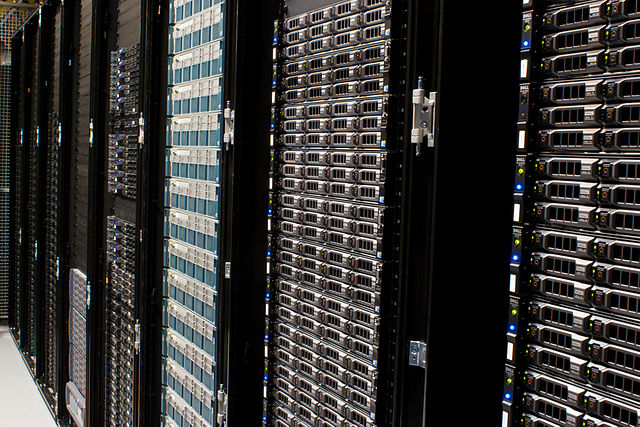
\includegraphics[width=3cm]{img/server.jpg}

			\small{x86, milliers d'unités}
		\end{center}
	}
	\end{minipage}
	\begin{minipage}[t]{0.30\linewidth}
		\uncover<3->{
		\begin{center}
			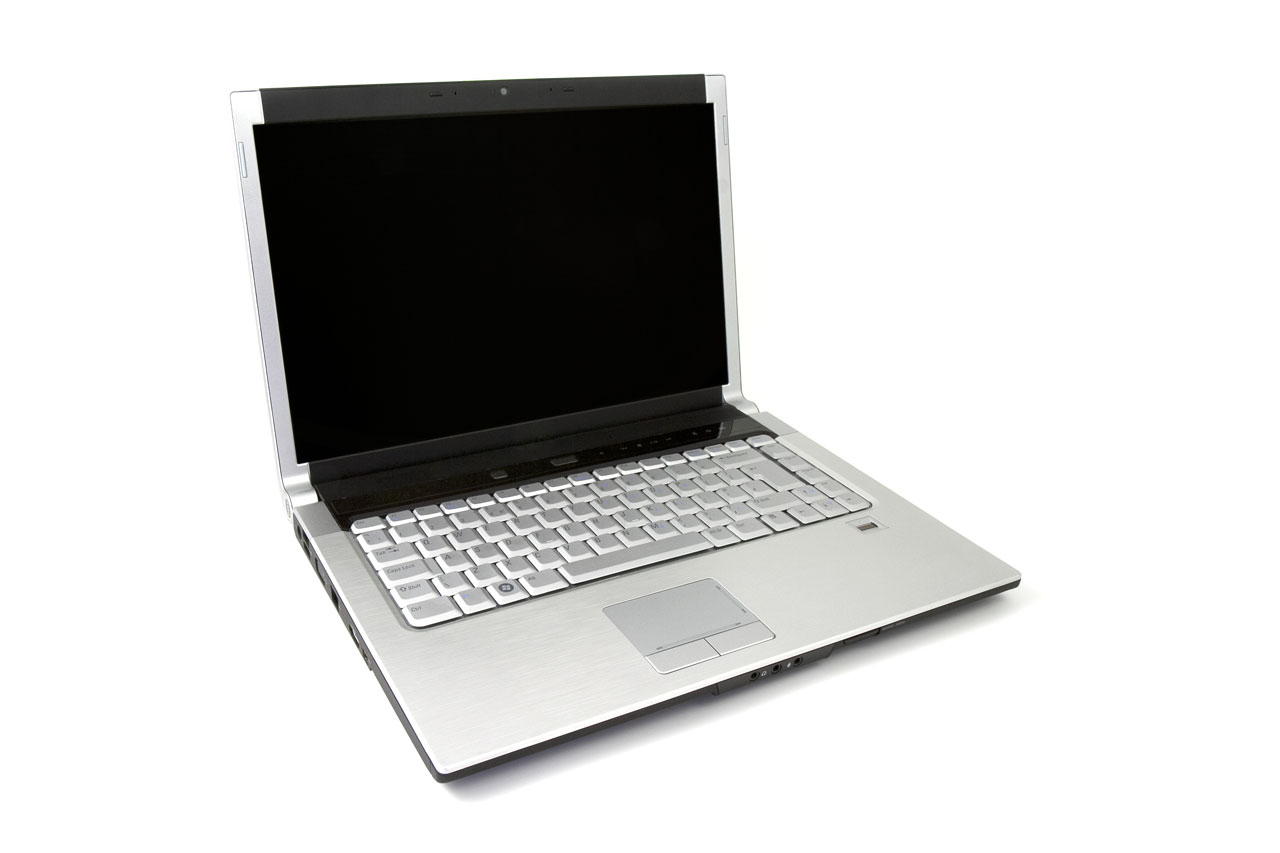
\includegraphics[width=3cm]{img/laptop.jpg}

			\small{x86, fléxibilité}
		\end{center}
	}
	\end{minipage}
	\begin{minipage}[t]{0.30\linewidth}
		\uncover<4->{
		\begin{center}
			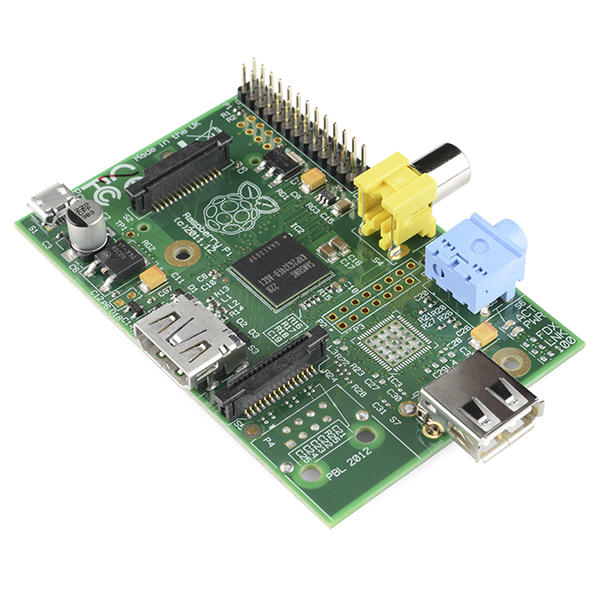
\includegraphics[width=3cm]{img/raspi.jpg}

			\small{ARM, autonomie}
		\end{center}
	}
	\end{minipage}
\end{frame}

